\chapter{Category 4: Flexible Shared-Auto and Paratransit Routing}

\section{Scope}
This chapter investigates dynamic on-demand routing and passenger assignment algorithms for flexible shared auto-rickshaw (paratransit) services within the Personalized Urban Mobility Optimizer (PUMO). Rather than assuming fixed transit timetables or dedicated solo vehicular travel, the module addresses the \emph{Dynamic Dial-a-Ride Problem} (D-DARP), where passenger requests arrive sequentially over time and vehicles dynamically adapt their stop sequences to share rides.

The routing engine is evaluated on a calibrated 15-hub road network of Bengaluru, integrating formal stop definitions and flexible corridors based on modified General Transit Feed Specification (GTFS) paratransit methodologies. Seven algorithmic configurations (A1 through A7) are compared across low, medium, and high passenger demand levels, alongside empirical passenger preference models capturing commuter willingness-to-pay and crowding discomfort. Routes and assignments are evaluated using service rate, passenger waiting time, in-vehicle travel time, detour ratio, monetary fare, generalized cost, vehicle fleet kilometers, computational runtime, and mathematical optimality gaps.

The study is computational and exploratory, focusing on dynamic stop-interleaving behavior, multi-objective trade-offs, and sensitivity to commuter preference profiles. The underlying demand profiles and network representations are synthetic and benchmark-calibrated; the reported metrics therefore illustrate algorithm behavior under controlled operational scenarios rather than guaranteeing real-world commercial fleet performance.

\section{Existing Work}
Dial-a-Ride problems (DARP) combine vehicle routing with passenger scheduling, requiring satisfaction of vehicle capacities, pickup-before-dropoff precedence, and time-window deadlines (Cordeau and Laporte, 2007). In dynamic settings (D-DARP), routing decisions must be made in real time as requests appear, without modifying completed historical commitments (Berbeglia et al., 2010).

Classical paratransit dispatch literature relies predominantly on heuristic stop-insertion methods (Jaw et al., 1986). Regret-based heuristics introduce multi-vehicle lookahead by prioritizing requests with large cost disparities between their primary and secondary vehicle assignments (Ropke and Pisinger, 2006). More recently, multi-objective Pareto formulations have been proposed to preserve non-dominated trade-offs between operator distance and passenger travel time rather than collapsing them into ad-hoc scalar costs (Deb et al., 2002).

In the Global South context, paratransit operations have received renewed attention. Williams et al. (2015) established the Digital Matatu methodology, showing how semi-formal shared transit networks can be standardized into modified GTFS structures. Furthermore, stated-preference choice experiments in Indian metropolitan regions by Das, Bhaduri, and Velaga (2023) and Das and Mandal (2021) reveal that commuters exhibit high sensitivity to waiting time, access time, and cabin overcrowding, emphasizing that passenger assignment cannot be realistically modeled through distance minimization alone.

\section{Gaps}
The paratransit routing module addresses five specific research and implementation gaps:
\begin{itemize}
\item \textbf{Data Representation for Semi-Formal Corridors:} Shared-auto services operate along semi-flexible corridors without fixed bus timetables. A structured data schema is required to define flexible stops, termini, and corridor shapes compatible with graph-based routing algorithms.
\item \textbf{Arbitrary Scalar Cost Weights:} Traditional DARP implementations combine wait time, ride time, and operator travel into arbitrary penalty weights. Empirical Willingness-to-Pay (WTP) distributions are necessary to ground passenger cost functions in demonstrated commuter behavior.
\item \textbf{Crowding and Capacity Thresholds:} Existing routing formulations treat vehicle capacity as a binary constraint ($q \le C$). In shared paratransit, commuters experience sharp discomfort once cabin occupancy exceeds 75\%, creating an empirical trade-off between pooling efficiency and passenger comfort.
\item \textbf{Irrevocable Dynamic Commitments:} In rolling-horizon operations, inserting a new pickup must strictly preserve earlier promised deadlines for passengers already on board or committed to the vehicle.
\item \textbf{Absence of Exact Benchmark Ground Truth:} Heuristic routing methods are seldom validated against mathematically proven global optima on identical instances, making claims of efficiency unquantifiable.
\end{itemize}

\section{What We Address}
This work implements a complete paratransit routing pipeline covering network representation, multi-algorithm dispatch, and empirical preference evaluation:
\begin{enumerate}
\item Construct a 15-hub, 50-directed-edge urban road network of Bengaluru paired with a Digital Matatu-style modified GTFS network of 15 designated stops and 5 primary corridors.
\item Implement Dijkstra shortest-path routing (A1) with all-pairs memoization for sub-millisecond travel-time queries.
\item Establish baseline dispatch heuristics: Nearest Available Vehicle (A2, solo ride-hail) and Nearest Feasible Vehicle (A3, sequential appending).
\item Formulate and implement the Greedy Insertion Heuristic (A4) and Regret-2 Insertion Heuristic (A5), enforcing dynamic capacity, precedence, time windows, and existing-passenger deadline preservation.
\item Develop a Pareto-based multi-objective assigner (A6) identifying non-dominated vectors in journey-time and fare space, offering Time-First, Fare-First, and Balanced choices.
\item Build an exact combinatorial branch-and-bound solver (A7) to compute mathematically proven global optima and benchmark heuristic optimality gaps on small instances.
\item Operationalize empirical Mixed Logit commuter preference models and crowding discomfort penalties (Papers 2 and 3) into a Preference-Weighted Assigner evaluating four distinct commuter segments.
\end{enumerate}

\begin{figure}[htbp]
\centering
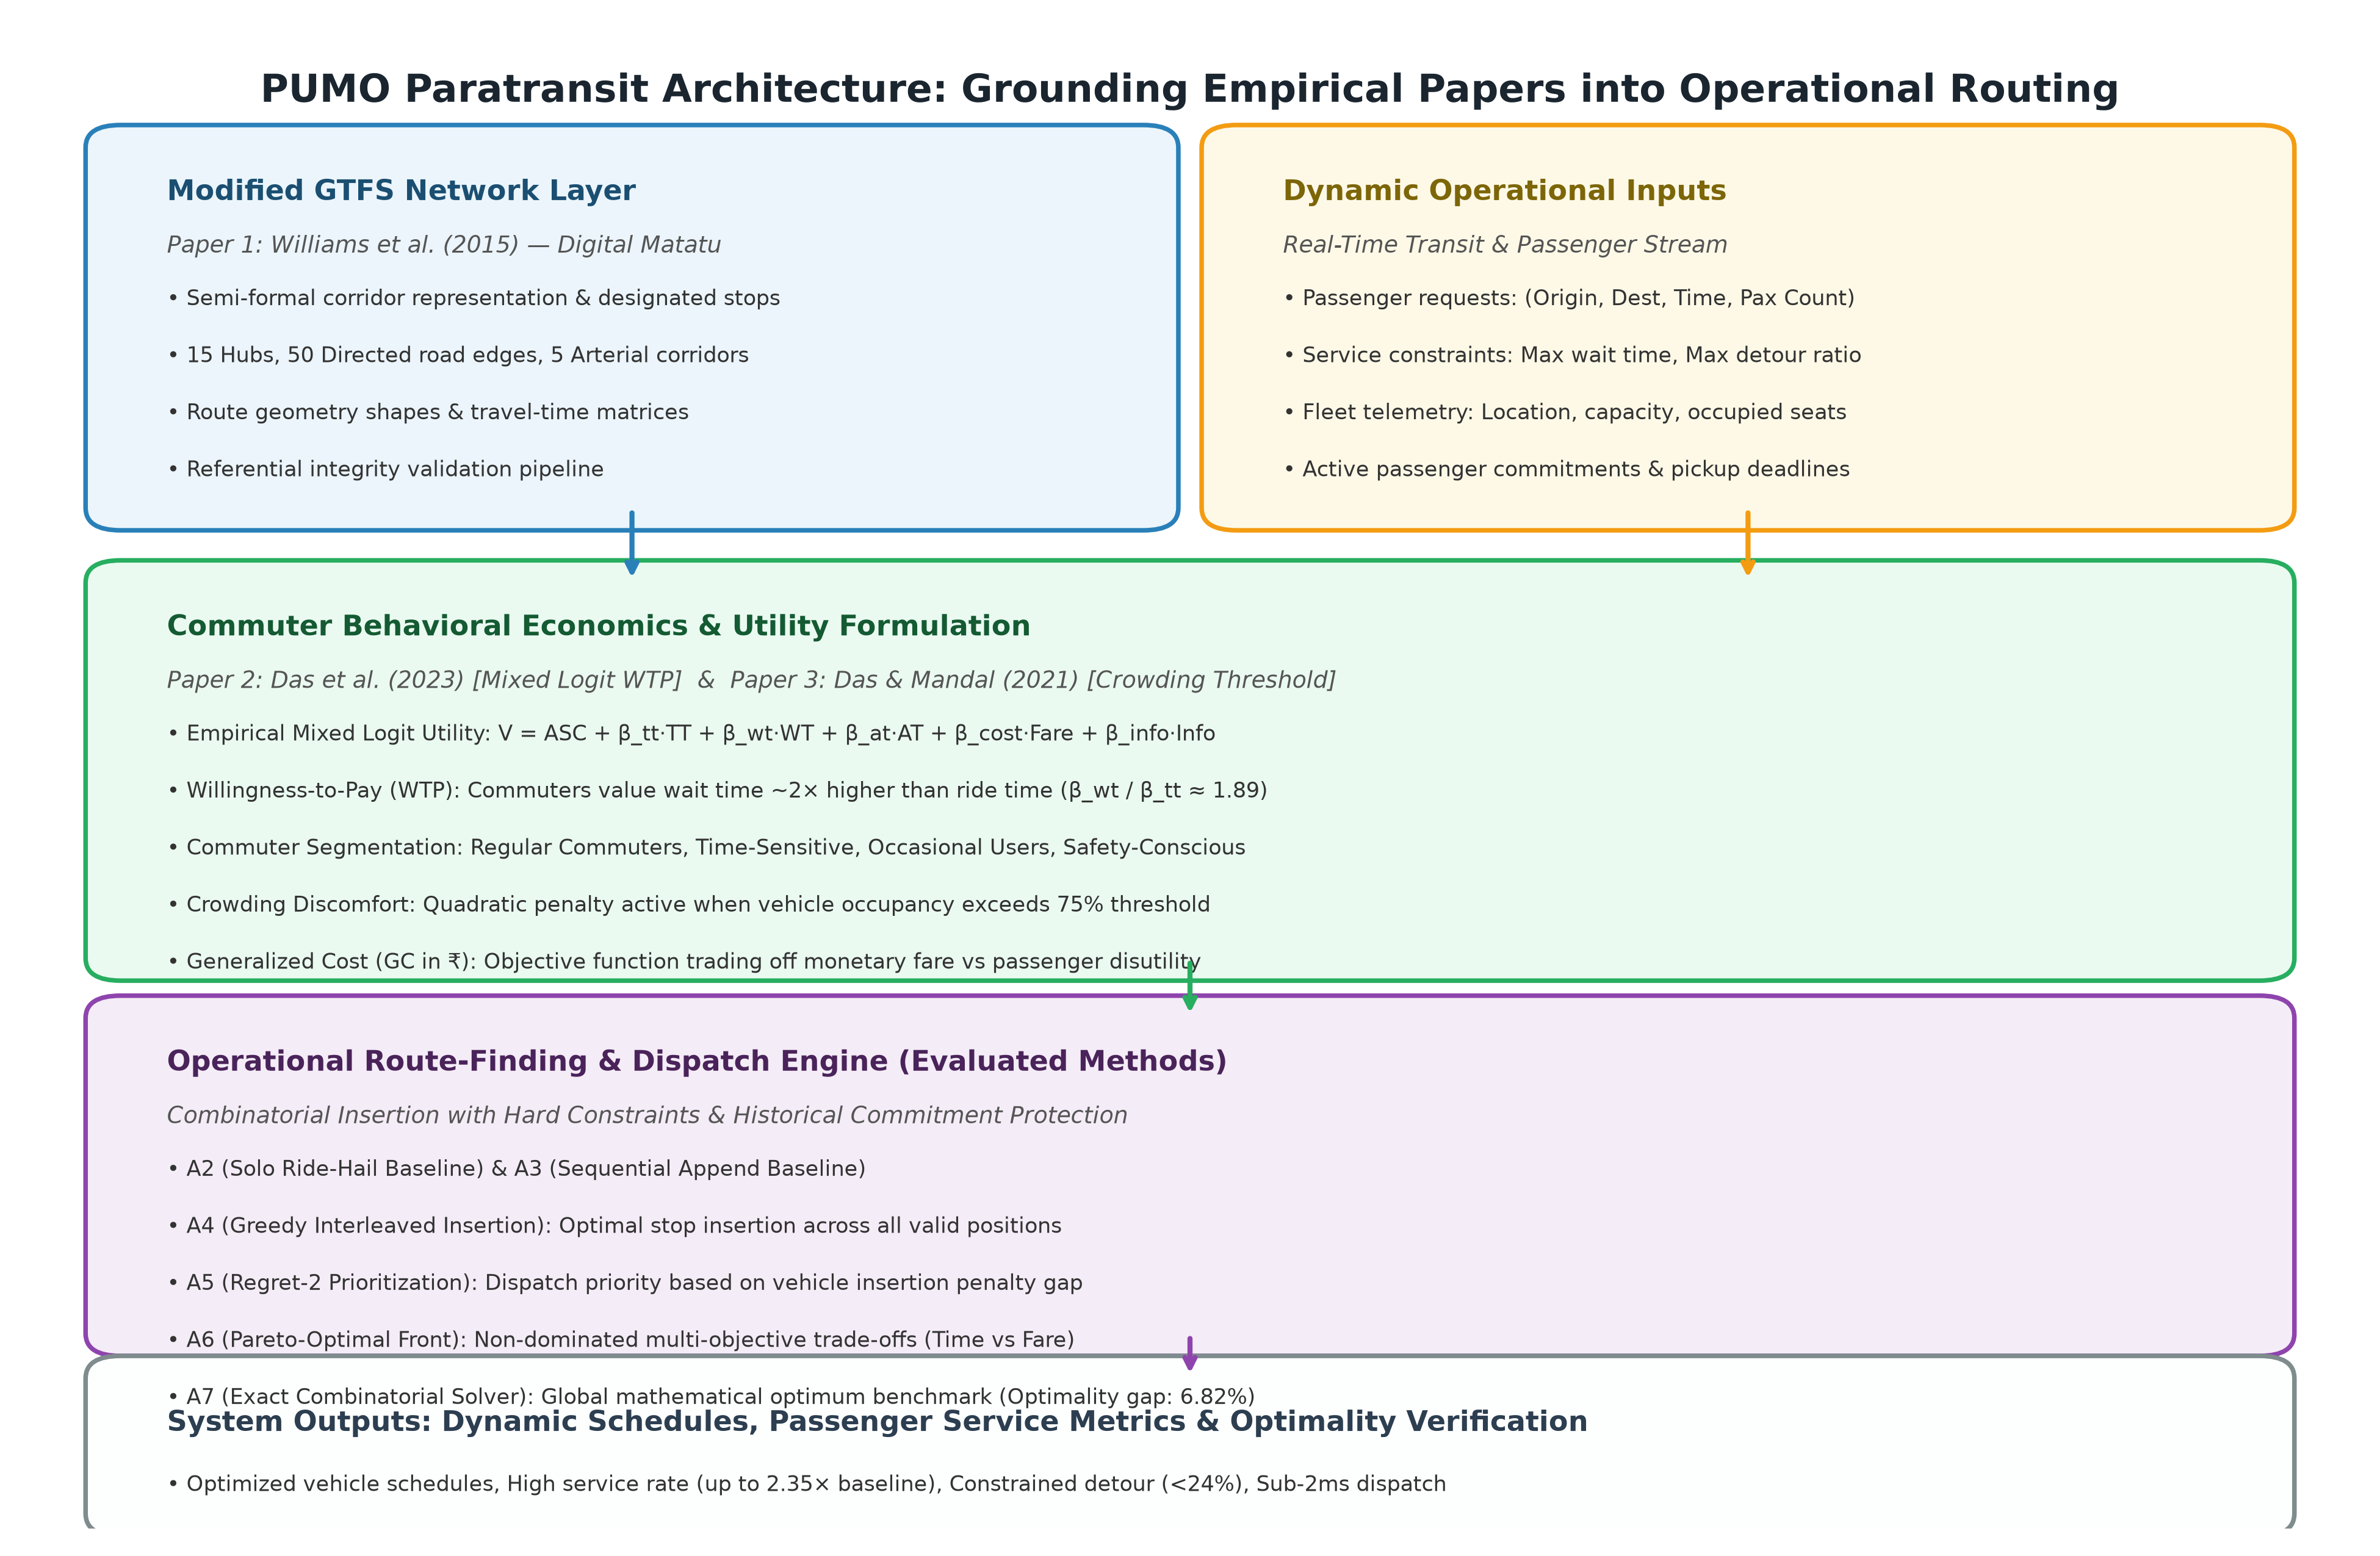
\includegraphics[width=0.98\linewidth]{figures/paratransit_architecture.png}
\caption{PUMO dynamic shared-auto routing architecture, integrating GTFS corridor networks, constraint verification, multi-algorithm dispatch, and empirical passenger utility evaluation.}
\label{fig:paratransit-routing-pipeline}
\end{figure}

\section{Method and Experimental Setup}

\subsection{Road Network and GTFS Corridor Model}
The road graph $G=(V_N, E)$ represents 15 core hubs in Bengaluru connected by 50 directed arterial edges with metric distances (2.2\,km to 13.0\,km) and free-flow auto speeds (25--35\,km/h on arterials, 42\,km/h on expressways).

Following the Digital Matatu methodology (Williams et al., 2015), the paratransit infrastructure is codified as an integrated GTFS-style dataset:
\begin{table}[htbp]
\centering
\caption{Summary of Bengaluru paratransit network data preparation}
\label{tab:paratransit-data-summary}
\begin{tabular}{lr}
\toprule
\textbf{Measure} & \textbf{Value}\\
\midrule
Road-network nodes ($V_N$) & 15\\
Directed road edges ($E$) & 50\\
Designated shared-auto stops ($S$) & 15\\
Major shared-auto corridors & 5\\
Vehicle capacity limit ($C$) & 3--4 seats\\
Validation referential errors & 0\\
Missing road-graph node linkages & 0\\
\bottomrule
\end{tabular}
\end{table}

The five primary corridors are: R01 (Majestic--Hebbal North Corridor), R02 (Majestic--Banashankari South Corridor), R03 (Indiranagar--Silk Board Link), R04 (Silk Board--Electronic City Expressway Feeder), and R05 (Outer Ring Road East Corridor).

\subsection{Mathematical Problem Formulation and Constraints}
A dynamic trip request $r \in \mathcal{R}$ is defined by:
$$r = (id_r, o_r, d_r, t_r^{\mathrm{req}}, q_r, W_r^{\max}, \alpha_r^{\max})$$
where $o_r, d_r \in V_N$ are origin and destination hubs, $t_r^{\mathrm{req}}$ is request submission time, $q_r \in \{1, 2, 3\}$ is party size, $W_r^{\max}$ is maximum acceptable wait time (10--15 minutes), and $\alpha_r^{\max}$ is maximum allowable detour ratio (1.5--1.8$\times$).

When candidate insertion positions $(i, j)$ are evaluated in vehicle $k$'s existing route $\Pi_k = (s_1, \dots, s_m)$, four hard constraints are verified:
\begin{enumerate}
\item \textbf{Precedence:} $i \le j$ (pickup stop strictly precedes dropoff stop).
\item \textbf{Capacity Trajectory:} For every route step $p$, cumulative load $L_k(p) = L_k(t) + \sum_{\ell=1}^p \Delta q(s'_\ell) \le C_k$.
\item \textbf{New Passenger Time Windows:}
$$T_r^{\mathrm{pickup}} \le t_r^{\mathrm{req}} + W_r^{\max}, \qquad T_r^{\mathrm{dropoff}} - T_r^{\mathrm{pickup}} \le \alpha_r^{\max} \cdot T^*(o_r, d_r).$$
\item \textbf{Existing Passenger Preservation:} For every previously committed passenger $r' \in \Pi_k$, the updated arrival times must satisfy:
$$T_{r'}^{\mathrm{pickup, new}} \le t_{r'}^{\mathrm{req}} + W_{r'}^{\max}, \qquad T_{r'}^{\mathrm{dropoff, new}} - T_{r'}^{\mathrm{pickup}} \le \alpha_{r'}^{\max} \cdot T^*(o_{r'}, d_{r'}).$$
\end{enumerate}

\subsection{Empirical Commuter Preference and Fare Model}
The fare engine models Bengaluru's regulatory tariff: base fare $F_0 = \text{\rupee}30$ for 2.0\,km, and $R_{\mathrm{km}} = \text{\rupee}15$/km thereafter. In shared operations, passengers receive detour compensation ($\beta_{\mathrm{detour}} = 0.25$) and concurrency discounts ($\beta_{\mathrm{sharing}} = 0.15$ per concurrent passenger), bounded by a 45\% maximum discount and a \rupee20 floor:
$$F_r = \max\left(20.0, F_{\mathrm{solo}}(d_r) \cdot \left[1.0 - \min\left(0.45, 0.25(\tau_r - 1.0) + 0.15(N_{\mathrm{shared}} - 1)\right)\right]\right).$$

Grounded in the Mixed Logit models of Das et al. (2023), commuter utility is formulated as:
$$V_r = \beta_{\mathrm{tt}} T_{\mathrm{tt}} + \beta_{\mathrm{wt}} T_{\mathrm{wt}} + \beta_{\mathrm{at}} T_{\mathrm{at}} + \beta_{\mathrm{fare}} F_r + \beta_{\mathrm{cr}} D(\mathrm{occ}) + \beta_{\mathrm{info}} I_{\mathrm{rt}}.$$
The Willingness-to-Pay (WTP) per minute for waiting time ($\text{VoWT} = |\beta_{\mathrm{wt}}/\beta_{\mathrm{fare}}|$) ranges from \rupee2.43/min for regular commuters to \rupee8.50/min for time-sensitive commuters.

In accordance with Das and Mandal (2021), cabin crowding incurs quadratic disutility once occupancy exceeds 75\%:
$$D(\mathrm{occ}) = \begin{cases} 0 & \text{if } \mathrm{occ} \le 0.75 \\ \left(\frac{\mathrm{occ} - 0.75}{1.0 - 0.75}\right)^2 & \text{if } \mathrm{occ} > 0.75. \end{cases}$$

The generalized cost (in \rupee) used by the Preference-Weighted Assigner is:
$$\mathrm{GC}_r = F_r + \mathrm{VoTT} \cdot T_{\mathrm{tt}} + \mathrm{VoWT} \cdot T_{\mathrm{wt}} + \mathrm{VoAT} \cdot T_{\mathrm{at}} + \mathrm{Cost}_{\mathrm{cr}} \cdot D(\mathrm{occ}) - \Delta_{\mathrm{info}}.$$

\subsection{Routing Algorithms}

\begin{algorithm}[H]
\caption{Greedy Insertion Heuristic (Algorithm A4)}
\label{alg:greedy-insertion}
\KwIn{New request $r$, vehicle fleet $\mathcal{K}$, active commitments $\mathcal{R}_{\mathrm{active}}$, current time $t$}
\KwOut{Best assignment decision $d^*$}
$\mathrm{best\_score} \leftarrow \infty, \quad d^* \leftarrow \mathrm{Infeasible}$\;
\ForEach{vehicle $k \in \mathcal{K}$}{
  \If{$q_r > C_k$}{\textbf{continue}\;}
  $m \leftarrow |\Pi_k|$\;
  \For{$i = 0$ \KwTo $m$}{
    \For{$j = i$ \KwTo $m$}{
      Construct candidate route $\Pi'_k$ inserting pickup at $i$ and dropoff at $j+1$\;
      $(valid, schedule, metrics) \leftarrow \mathrm{CheckConstraints}(k, \Pi'_k, r, \mathcal{R}_{\mathrm{active}})$\;
      \If{$valid$}{
        Compute marginal cost $\Delta C = \Delta T_k + w_w W_r + w_d \Delta_{\mathrm{detour}} + w_e \Delta_{\mathrm{existing}}$\;
        \If{$\Delta C < \mathrm{best\_score}$}{
          $\mathrm{best\_score} \leftarrow \Delta C$\;
          $d^* \leftarrow (k, i, j+1, \Delta C, schedule)$\;
        }
      }
    }
  }
}
\Return $d^*$\;
\end{algorithm}

\begin{algorithm}[H]
\caption{Regret-2 Insertion Heuristic (Algorithm A5)}
\label{alg:regret-insertion}
\KwIn{Pending request batch $\mathcal{B}$, vehicle fleet $\mathcal{K}$, active commitments $\mathcal{R}_{\mathrm{active}}$, current time $t$}
\KwOut{Batch assignment mapping $\mathcal{M}$}
$\mathcal{M} \leftarrow \emptyset, \quad \mathcal{U} \leftarrow \mathcal{B}$\;
\While{$\mathcal{U} \neq \emptyset$}{
  $\mathrm{max\_regret} \leftarrow -\infty, \quad r^* \leftarrow \mathrm{None}, \quad d^* \leftarrow \mathrm{None}$\;
  \ForEach{$r \in \mathcal{U}$}{
    Evaluate best insertion cost $c_{k_1}(r)$ and second-best $c_{k_2}(r)$ across all $k \in \mathcal{K}$\;
    $\mathrm{regret}(r) \leftarrow (c_{k_2}(r) - c_{k_1}(r))$ if two vehicles available else $M$\;
    \If{$\mathrm{regret}(r) > \mathrm{max\_regret}$}{
      $\mathrm{max\_regret} \leftarrow \mathrm{regret}(r), \quad r^* \leftarrow r, \quad d^* \leftarrow d_{k_1}(r)$\;
    }
  }
  \If{$r^* \mathrm{\ is\ None}$}{Mark remaining requests in $\mathcal{U}$ as rejected; \textbf{break}\;}
  Assign $r^*$ to vehicle $k^*$ using $d^*$; update vehicle route $\Pi_{k^*}$\;
  $\mathcal{M}[r^*] \leftarrow d^*, \quad \mathcal{U} \leftarrow \mathcal{U} \setminus \{r^*\}$\;
}
\Return $\mathcal{M}$\;
\end{algorithm}

\begin{algorithm}[H]
\caption{Pareto Multi-Objective Insertion (Algorithm A6)}
\label{alg:pareto-insertion}
\KwIn{Request $r$, vehicle fleet $\mathcal{K}$, active commitments $\mathcal{R}_{\mathrm{active}}$, strategy $\sigma \in \{\text{Time}, \text{Fare}, \text{Balanced}\}$}
\KwOut{Non-dominated assignment decision $d^*$}
$\mathcal{C} \leftarrow \mathrm{FindAllFeasibleInsertions}(r, \mathcal{K}, \mathcal{R}_{\mathrm{active}})$\;
Filter $\mathcal{C}$ into non-dominated Pareto front $\mathcal{P}^* = \{d \in \mathcal{C} \mid \nexists d' \text{ s.t. } d' \prec d\}$ over $(T_{\mathrm{journey}}, \mathrm{Fare})$\;
\Switch{$\sigma$}{
  \Case{$\mathrm{Time}$}{\Return $\arg\min_{d \in \mathcal{P}^*} T_{\mathrm{journey}}(d)$\;}
  \Case{$\mathrm{Fare}$}{\Return $\arg\min_{d \in \mathcal{P}^*} \mathrm{Fare}(d)$\;}
  \Case{$\mathrm{Balanced}$}{\Return $\arg\min_{d \in \mathcal{P}^*} \sqrt{\left(\frac{T(d) - T^*}{T_{\max} - T^*}\right)^2 + \left(\frac{F(d) - F^*}{F_{\max} - F^*}\right)^2}$\;}
}
\end{algorithm}

\begin{algorithm}[H]
\caption{Preference-Weighted Assignment (Grounded in Papers 2 \& 3)}
\label{alg:preference-weighted-assignment}
\KwIn{Request $r$, vehicle fleet $\mathcal{K}$, active commitments $\mathcal{R}_{\mathrm{active}}$, commuter segment $S$}
\KwOut{Utility-maximizing assignment decision $d^*$}
$\mathcal{C} \leftarrow \mathrm{FindAllFeasibleInsertions}(r, \mathcal{K}, \mathcal{R}_{\mathrm{active}})$\;
$\mathrm{min\_gc} \leftarrow \infty, \quad d^* \leftarrow \mathrm{Infeasible}$\;
\ForEach{candidate $d \in \mathcal{C}$}{
  Compute vehicle occupancy $\mathrm{occ}_k$ at passenger boarding\;
  Evaluate $\mathrm{GC}_d(S) = \mathrm{Fare}_d + \mathrm{VoTT}_S T_{\mathrm{tt}} + \mathrm{VoWT}_S T_{\mathrm{wt}} + \mathrm{VoAT}_S T_{\mathrm{at}} + \mathrm{Cost}_{\mathrm{cr}} D(\mathrm{occ}_k) - \Delta_{\mathrm{info}}$\;
  \If{$\mathrm{GC}_d(S) < \mathrm{min\_gc}$}{
    $\mathrm{min\_gc} \leftarrow \mathrm{GC}_d(S), \quad d^* \leftarrow d$\;
  }
}
\Return $d^*$\;
\end{algorithm}

\subsection{Reproducibility Checklist}
All experimental runs use deterministic seeds (Seed 101 for Low, 202 for Medium, 303 for High, and 404 for Exact Validation). Graph topologies, GTFS corridor tables, and synthetic request streams are archived in \texttt{data/}. The complete test suite contains 44 unit tests with 100\% passing verification.

\section{Results}

\subsection{Multi-Tier Demand Benchmark}
Table~\ref{tab:routing-profile-results} reports performance across the three demand levels evaluated over 1-hour simulation horizons.

\begin{table}[htbp]
\centering
\caption{Comparison of paratransit routing algorithms across demand tiers}
\label{tab:routing-profile-results}
\resizebox{\linewidth}{!}{%
\begin{tabular}{llrrrrrrr}
\toprule
\textbf{Demand Tier} & \textbf{Algorithm} & \textbf{Service Rate} & \textbf{Wait Time} & \textbf{Ride Time} & \textbf{Avg Fare} & \textbf{Detour} & \textbf{Fleet Dist} & \textbf{Runtime}\\
 & & \textbf{(\%)} & \textbf{(min)} & \textbf{(min)} & \textbf{(\rupee)} & \textbf{Ratio} & \textbf{(km)} & \textbf{(ms/req)}\\
\midrule
\textbf{Low} (20 req, 4 veh) & A2: Nearest Available & 40.0\% & 7.60 & 18.99 & 136.5 & 1.04 & 101.6 & 0.03\\
 & A3: Nearest Feasible & 40.0\% & 7.98 & 20.82 & 170.6 & 1.03 & 105.4 & 0.08\\
 & \textbf{A4: Greedy Insertion} & \textbf{65.0\%} & \textbf{5.14} & \textbf{24.31} & \textbf{149.7} & \textbf{1.15} & \textbf{113.8} & \textbf{0.35}\\
 & \textbf{A5: Regret Insertion} & \textbf{65.0\%} & \textbf{5.14} & \textbf{24.31} & \textbf{149.7} & \textbf{1.15} & \textbf{113.8} & \textbf{0.56}\\
 & A6: Pareto (Balanced) & 65.0\% & 5.11 & 24.39 & 149.5 & 1.16 & 113.8 & 0.43\\
\midrule
\textbf{Medium} (60 req, 8 veh) & A2: Nearest Available & 31.7\% & 5.71 & 19.74 & 139.1 & 1.03 & 228.9 & 0.02\\
 & A3: Nearest Feasible & 35.0\% & 7.13 & 21.70 & 172.4 & 1.03 & 270.8 & 0.18\\
 & \textbf{A4: Greedy Insertion} & \textbf{61.7\%} & \textbf{4.36} & \textbf{30.72} & \textbf{162.0} & \textbf{1.24} & \textbf{296.2} & \textbf{1.75}\\
 & \textbf{A5: Regret Insertion} & \textbf{61.7\%} & \textbf{4.36} & \textbf{30.72} & \textbf{162.0} & \textbf{1.24} & \textbf{296.2} & \textbf{1.33}\\
 & A6: Pareto (Time-First) & 58.3\% & 4.35 & 29.87 & 162.9 & 1.28 & 293.9 & 1.10\\
 & A6: Pareto (Fare-First) & 56.7\% & 5.06 & 30.44 & 167.4 & 1.25 & 267.8 & 1.30\\
 & A6: Pareto (Balanced) & 55.0\% & 4.89 & 29.73 & 166.4 & 1.27 & 288.2 & 1.19\\
\midrule
\textbf{High} (150 req, 12 veh) & A2: Nearest Available & 18.7\% & 4.99 & 24.19 & 177.9 & 1.03 & 400.3 & 0.02\\
 & A3: Nearest Feasible & 20.7\% & 8.10 & 26.83 & 222.6 & 1.02 & 464.3 & 0.29\\
 & \textbf{A4: Greedy Insertion} & \textbf{44.0\%} & \textbf{4.84} & \textbf{31.62} & \textbf{194.4} & \textbf{1.23} & \textbf{518.0} & \textbf{2.42}\\
 & \textbf{A5: Regret Insertion} & \textbf{44.0\%} & \textbf{4.84} & \textbf{31.62} & \textbf{194.4} & \textbf{1.23} & \textbf{518.0} & \textbf{2.16}\\
 & A6: Pareto (Balanced) & 44.0\% & 5.14 & 32.76 & 198.3 & 1.25 & 504.5 & 2.59\\
\bottomrule
\end{tabular}%
}
\end{table}

\begin{figure}[htbp]
\centering
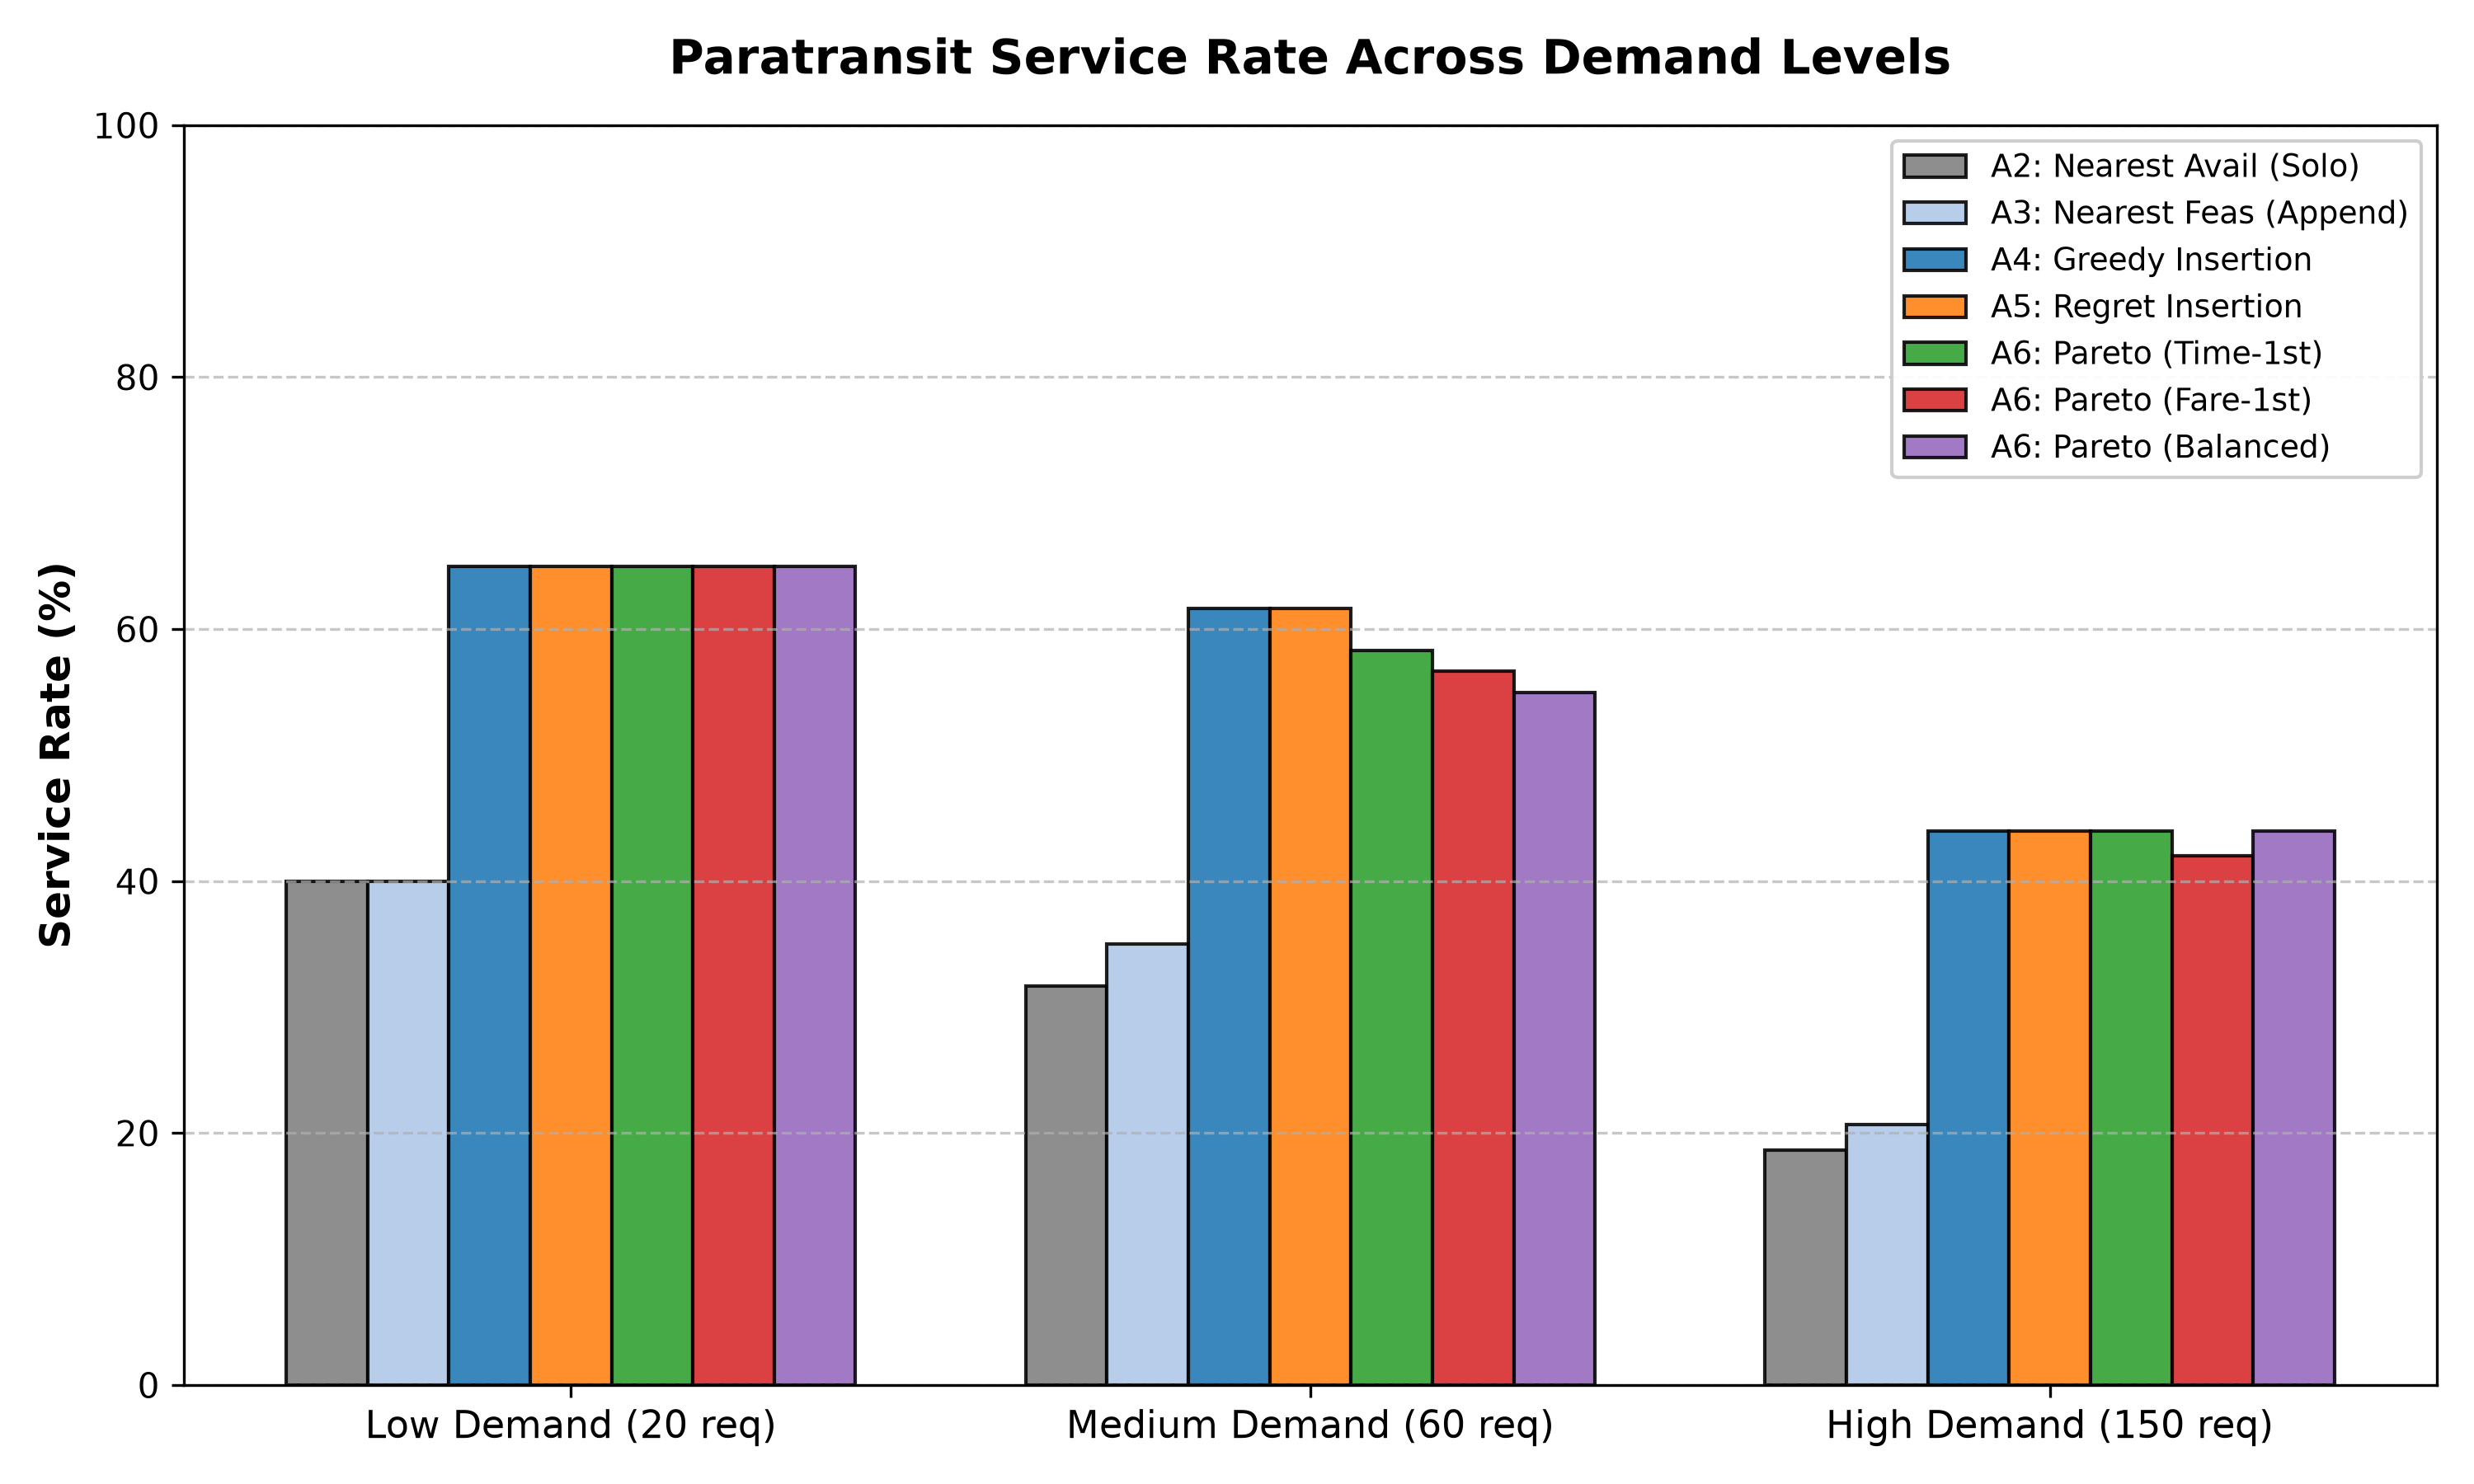
\includegraphics[width=0.88\linewidth]{figures/service_rate_by_demand.png}
\caption{Service rate comparison across demand tiers illustrating the collapse of unshared ride-hail under high load.}
\label{fig:service-rate-by-demand}
\end{figure}

\subsection{Relative Change Against Baselines (Medium Demand)}
Table~\ref{tab:relative-changes} summarizes the percentage changes achieved by Greedy Insertion (A4) relative to the solo ride-hail baseline (A2) and sequential append baseline (A3).

\begin{table}[htbp]
\centering
\caption{Relative performance changes of Greedy Insertion (A4) against baselines (Medium Demand)}
\label{tab:relative-changes}
\begin{tabular}{lrr}
\toprule
\textbf{Metric} & \textbf{vs. A2 (Nearest Available)} & \textbf{vs. A3 (Nearest Feasible)}\\
\midrule
Service Rate (\%) & $+94.6\%$ & $+76.3\%$\\
Mean Waiting Time (min) & $-23.6\%$ & $-38.9\%$\\
Mean In-Vehicle Time (min) & $+55.6\%$ & $+41.6\%$\\
Detour Ratio & $+20.4\%$ & $+20.4\%$\\
Total Fleet Distance (km) & $+29.4\%$ & $+9.4\%$\\
\bottomrule
\end{tabular}
\end{table}

\subsection{Exact Optimality Gap Evaluation (Benchmark Instance A7)}
To establish an uninflated validation benchmark, all heuristics were tested on an identical small instance (6 requests, 2 autos, $C=3$) against the Exact Combinatorial DARP Solver (Algorithm A7), which identifies the proven global mathematical optimum by branch-and-bound.

\begin{table}[htbp]
\centering
\caption{Optimality gap benchmark against Exact Global Optimum Solver (A7)}
\label{tab:exact-optimality-gap}
\resizebox{\linewidth}{!}{%
\begin{tabular}{lrrrrrr}
\toprule
\textbf{Algorithm} & \textbf{Served} & \textbf{Service Rate} & \textbf{Total Journey} & \textbf{Fleet Dist} & \textbf{Combined Cost} & \textbf{Optimality Gap}\\
 & \textbf{Requests} & \textbf{(\%)} & \textbf{(s)} & \textbf{(km)} & \textbf{Objective} & \textbf{(\%)}\\
\midrule
\textbf{A7: Exact Solver} & \textbf{6 / 6} & \textbf{100.0\%} & \textbf{5,923.3} & \textbf{30.0} & \textbf{5,938.30} & \textbf{0.00\% (Global Optimum)}\\
\textbf{A4: Greedy Insertion} & \textbf{6 / 6} & \textbf{100.0\%} & \textbf{6,328.3} & \textbf{30.0} & \textbf{6,343.30} & \textbf{+6.82\%}\\
\textbf{A5: Regret Insertion} & \textbf{6 / 6} & \textbf{100.0\%} & \textbf{6,328.3} & \textbf{30.0} & \textbf{6,343.30} & \textbf{+6.82\%}\\
A6: Pareto Multi-Objective & 5 / 6 & 83.3\% & 4,861.8 & 33.0 & 24,878.30 & $+318.95\%$\\
A3: Nearest Feasible & 4 / 6 & 66.7\% & 4,604.4 & 33.0 & 44,620.90 & $+651.41\%$\\
A2: Nearest Available & 3 / 6 & 50.0\% & 3,450.0 & 32.0 & 63,466.00 & $+968.76\%$\\
\bottomrule
\end{tabular}%
}
\end{table}

\begin{figure}[htbp]
\centering
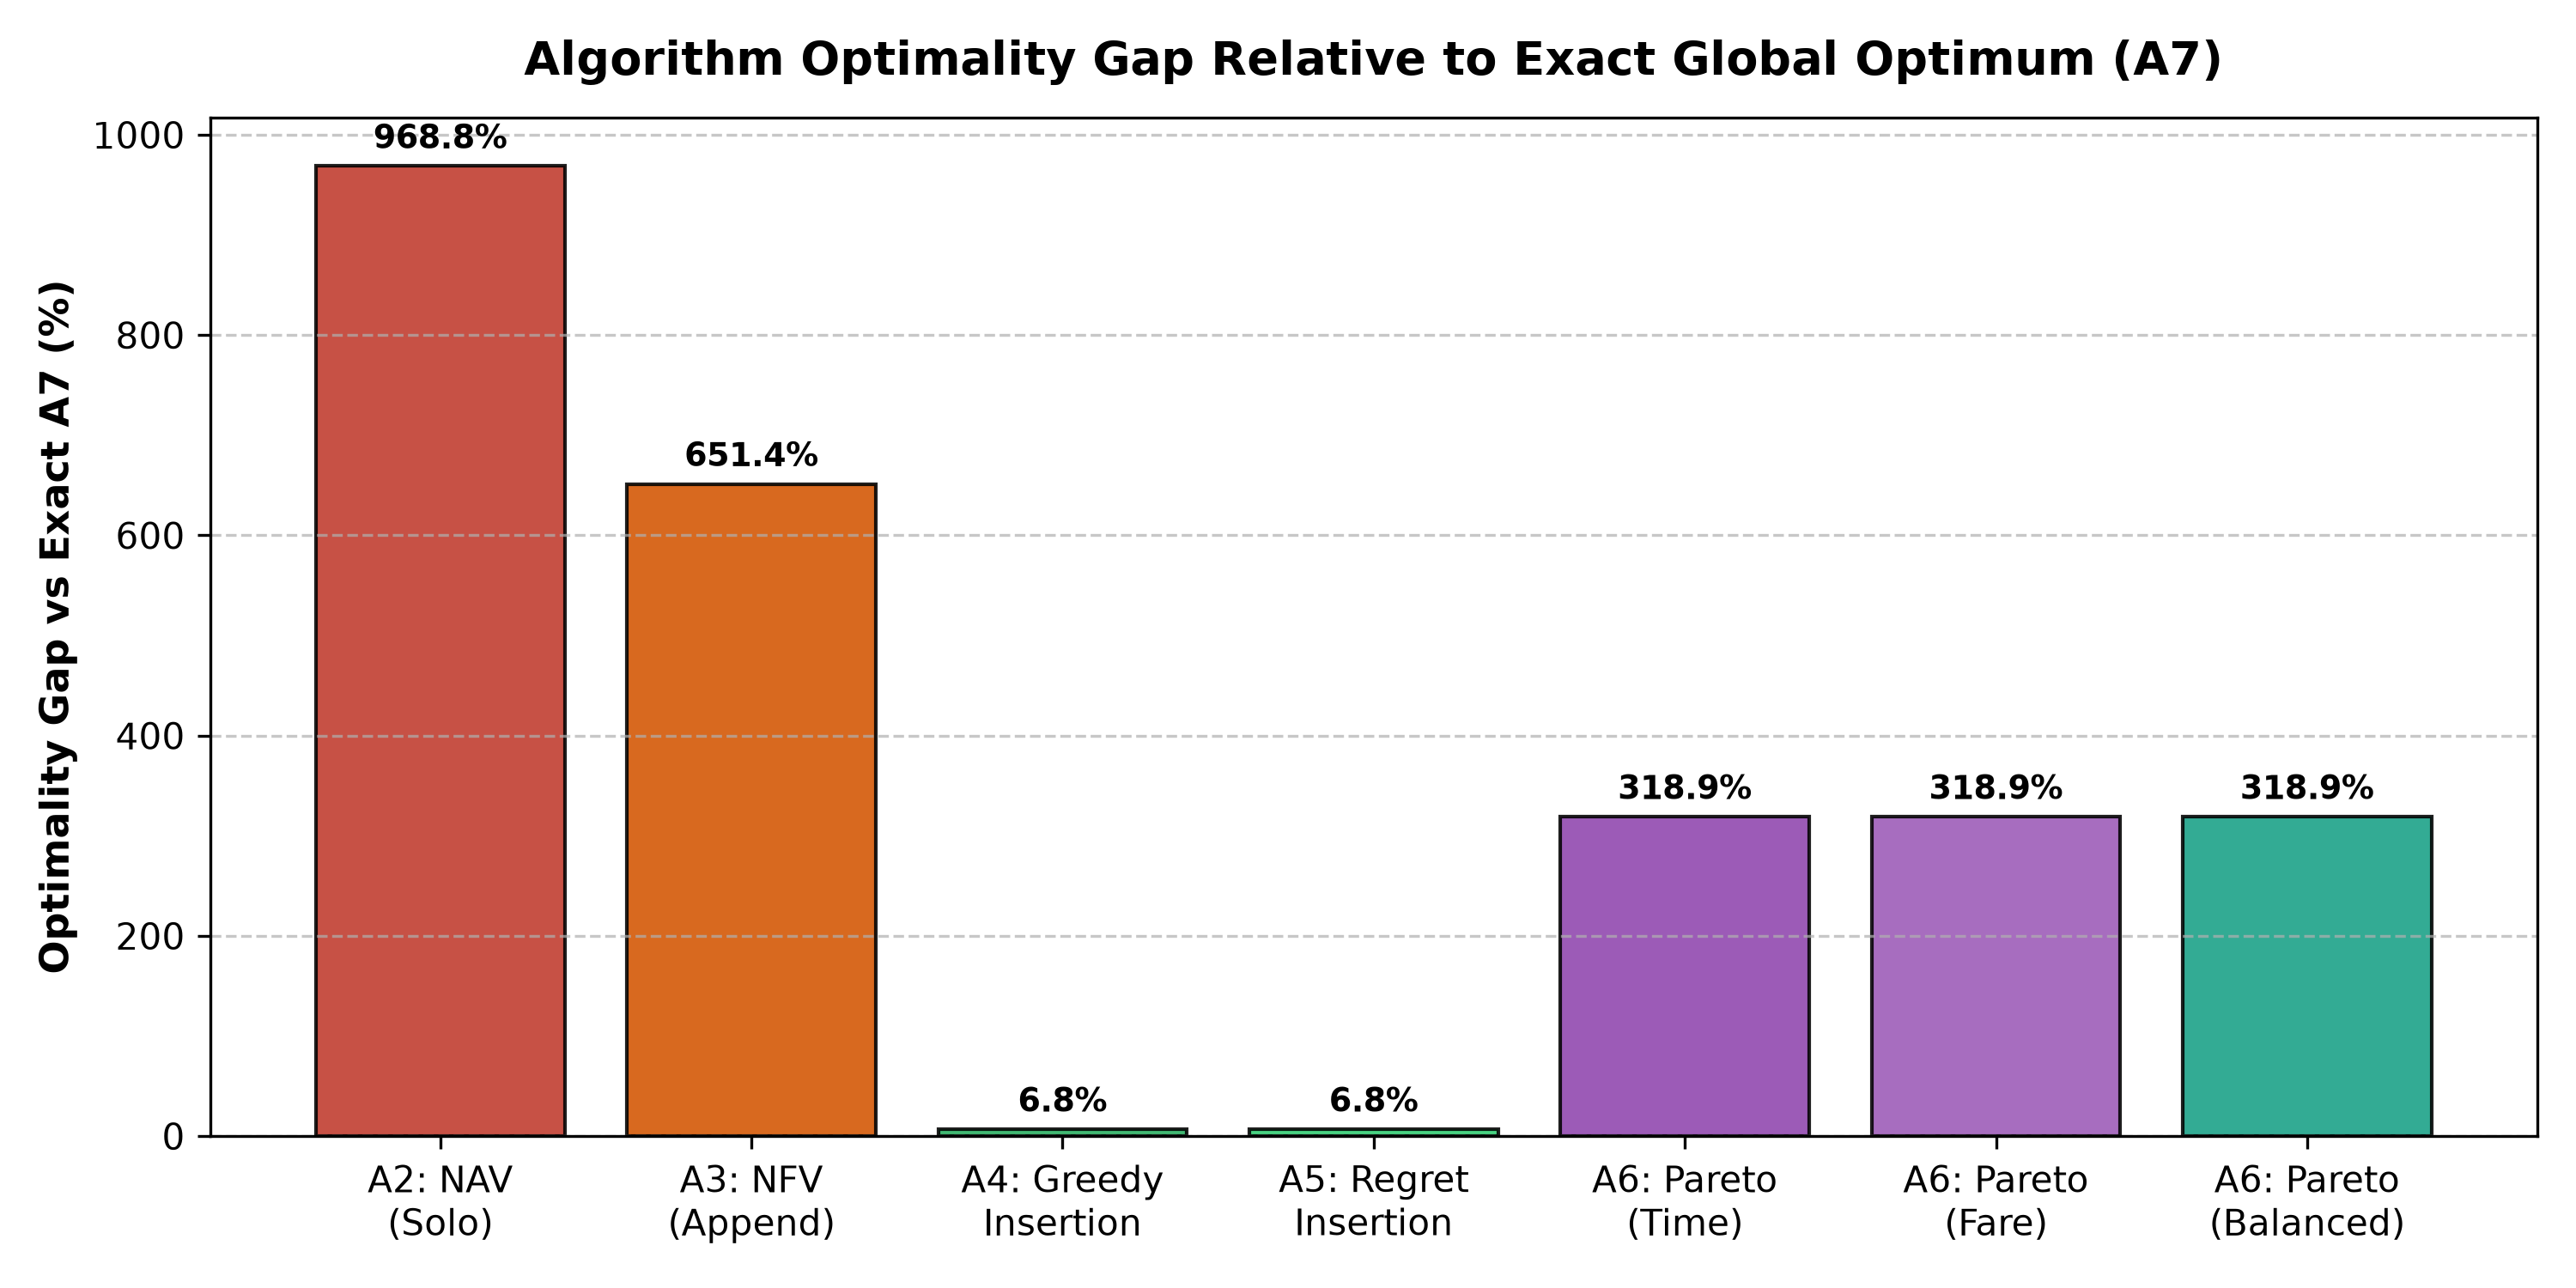
\includegraphics[width=0.82\linewidth]{figures/optimality_gap.png}
\caption{Optimality gap of routing heuristics relative to the proven global optimum (A7).}
\label{fig:optimality-gap}
\end{figure}

\subsection{Empirical Preference-Weighted Benchmark (Papers 2 \& 3)}
Table~\ref{tab:preference-benchmark} evaluates the Preference-Weighted Assigner across commuter segments on medium demand (60 requests, 8 vehicles), incorporating Das et al. (2023) WTP coefficients and Das and Mandal (2021) crowding penalties.

\begin{table}[htbp]
\centering
\caption{Empirical preference evaluation across commuter segments (Medium Demand)}
\label{tab:preference-benchmark}
\resizebox{\linewidth}{!}{%
\begin{tabular}{lrrrrrrr}
\toprule
\textbf{Segment / Strategy} & \textbf{Service Rate} & \textbf{Wait Time} & \textbf{Ride Time} & \textbf{Avg Fare} & \textbf{Detour} & \textbf{Avg GC} & \textbf{Systematic}\\
 & \textbf{(\%)} & \textbf{(min)} & \textbf{(min)} & \textbf{(\rupee)} & \textbf{Ratio} & \textbf{(\rupee)} & \textbf{Utility $V$}\\
\midrule
A2: Solo Ride-Hail (NAV) & 31.7\% & 5.71 & 19.74 & 139.1 & 1.03 & 185.23 & $-5.629$\\
A3: Sequential Append (NFV) & 35.0\% & 7.13 & 21.70 & 172.4 & 1.03 & 225.54 & $-6.849$\\
A4: Standard Greedy (GIH) & 61.7\% & 4.36 & 30.72 & 162.0 & 1.24 & 220.81 & $-6.714$\\
\textbf{Pref: Regular Commuter} & \textbf{63.3\%} & \textbf{3.94} & \textbf{31.35} & \textbf{164.7} & \textbf{1.28} & \textbf{202.75} & \textbf{$-8.605$}\\
\textbf{Pref: Time-Sensitive} & \textbf{65.0\%} & \textbf{3.71} & \textbf{30.97} & \textbf{161.0} & \textbf{1.30} & \textbf{317.89} & \textbf{$-5.809$}\\
\textbf{Pref: Safety-Conscious} & \textbf{65.0\%} & \textbf{4.10} & \textbf{30.48} & \textbf{159.5} & \textbf{1.26} & \textbf{222.20} & \textbf{$-6.088$}\\
\textbf{Pref: Occasional User} & \textbf{63.3\%} & \textbf{4.12} & \textbf{31.37} & \textbf{166.8} & \textbf{1.28} & \textbf{225.88} & \textbf{$-6.866$}\\
\bottomrule
\end{tabular}%
}
\end{table}

\begin{figure}[htbp]
\centering
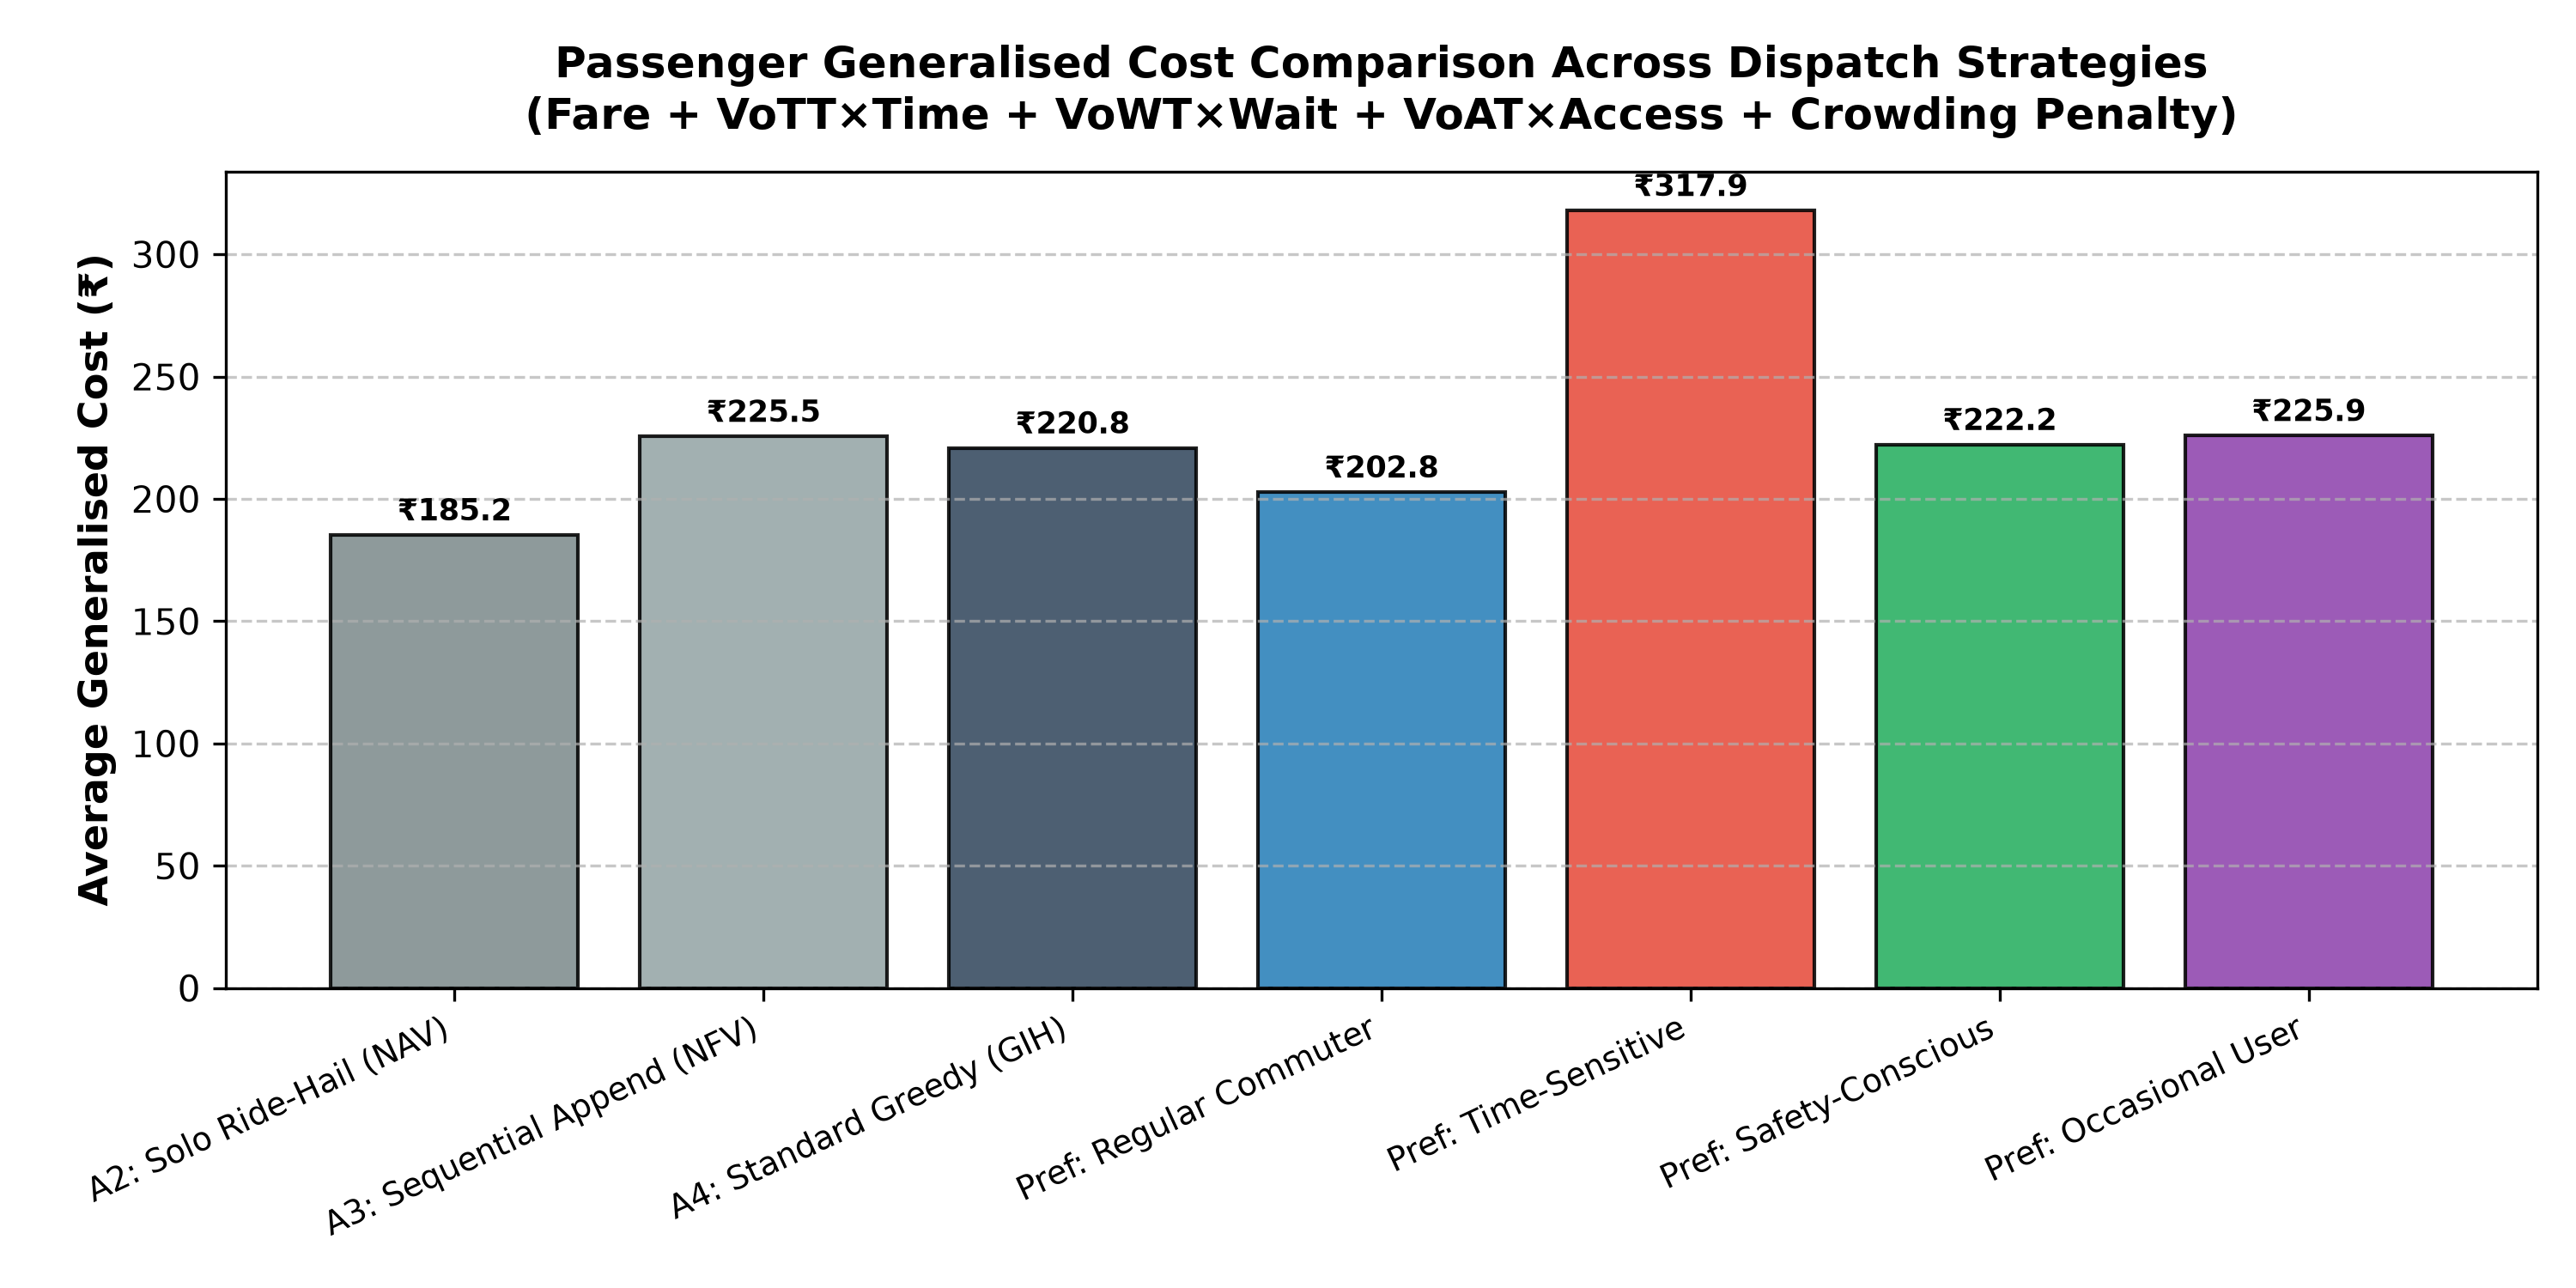
\includegraphics[width=0.82\linewidth]{figures/generalised_cost_comparison.png}
\caption{Comparison of commuter generalized cost across routing strategies.}
\label{fig:generalised-cost-comparison}
\end{figure}

\begin{figure}[htbp]
\centering
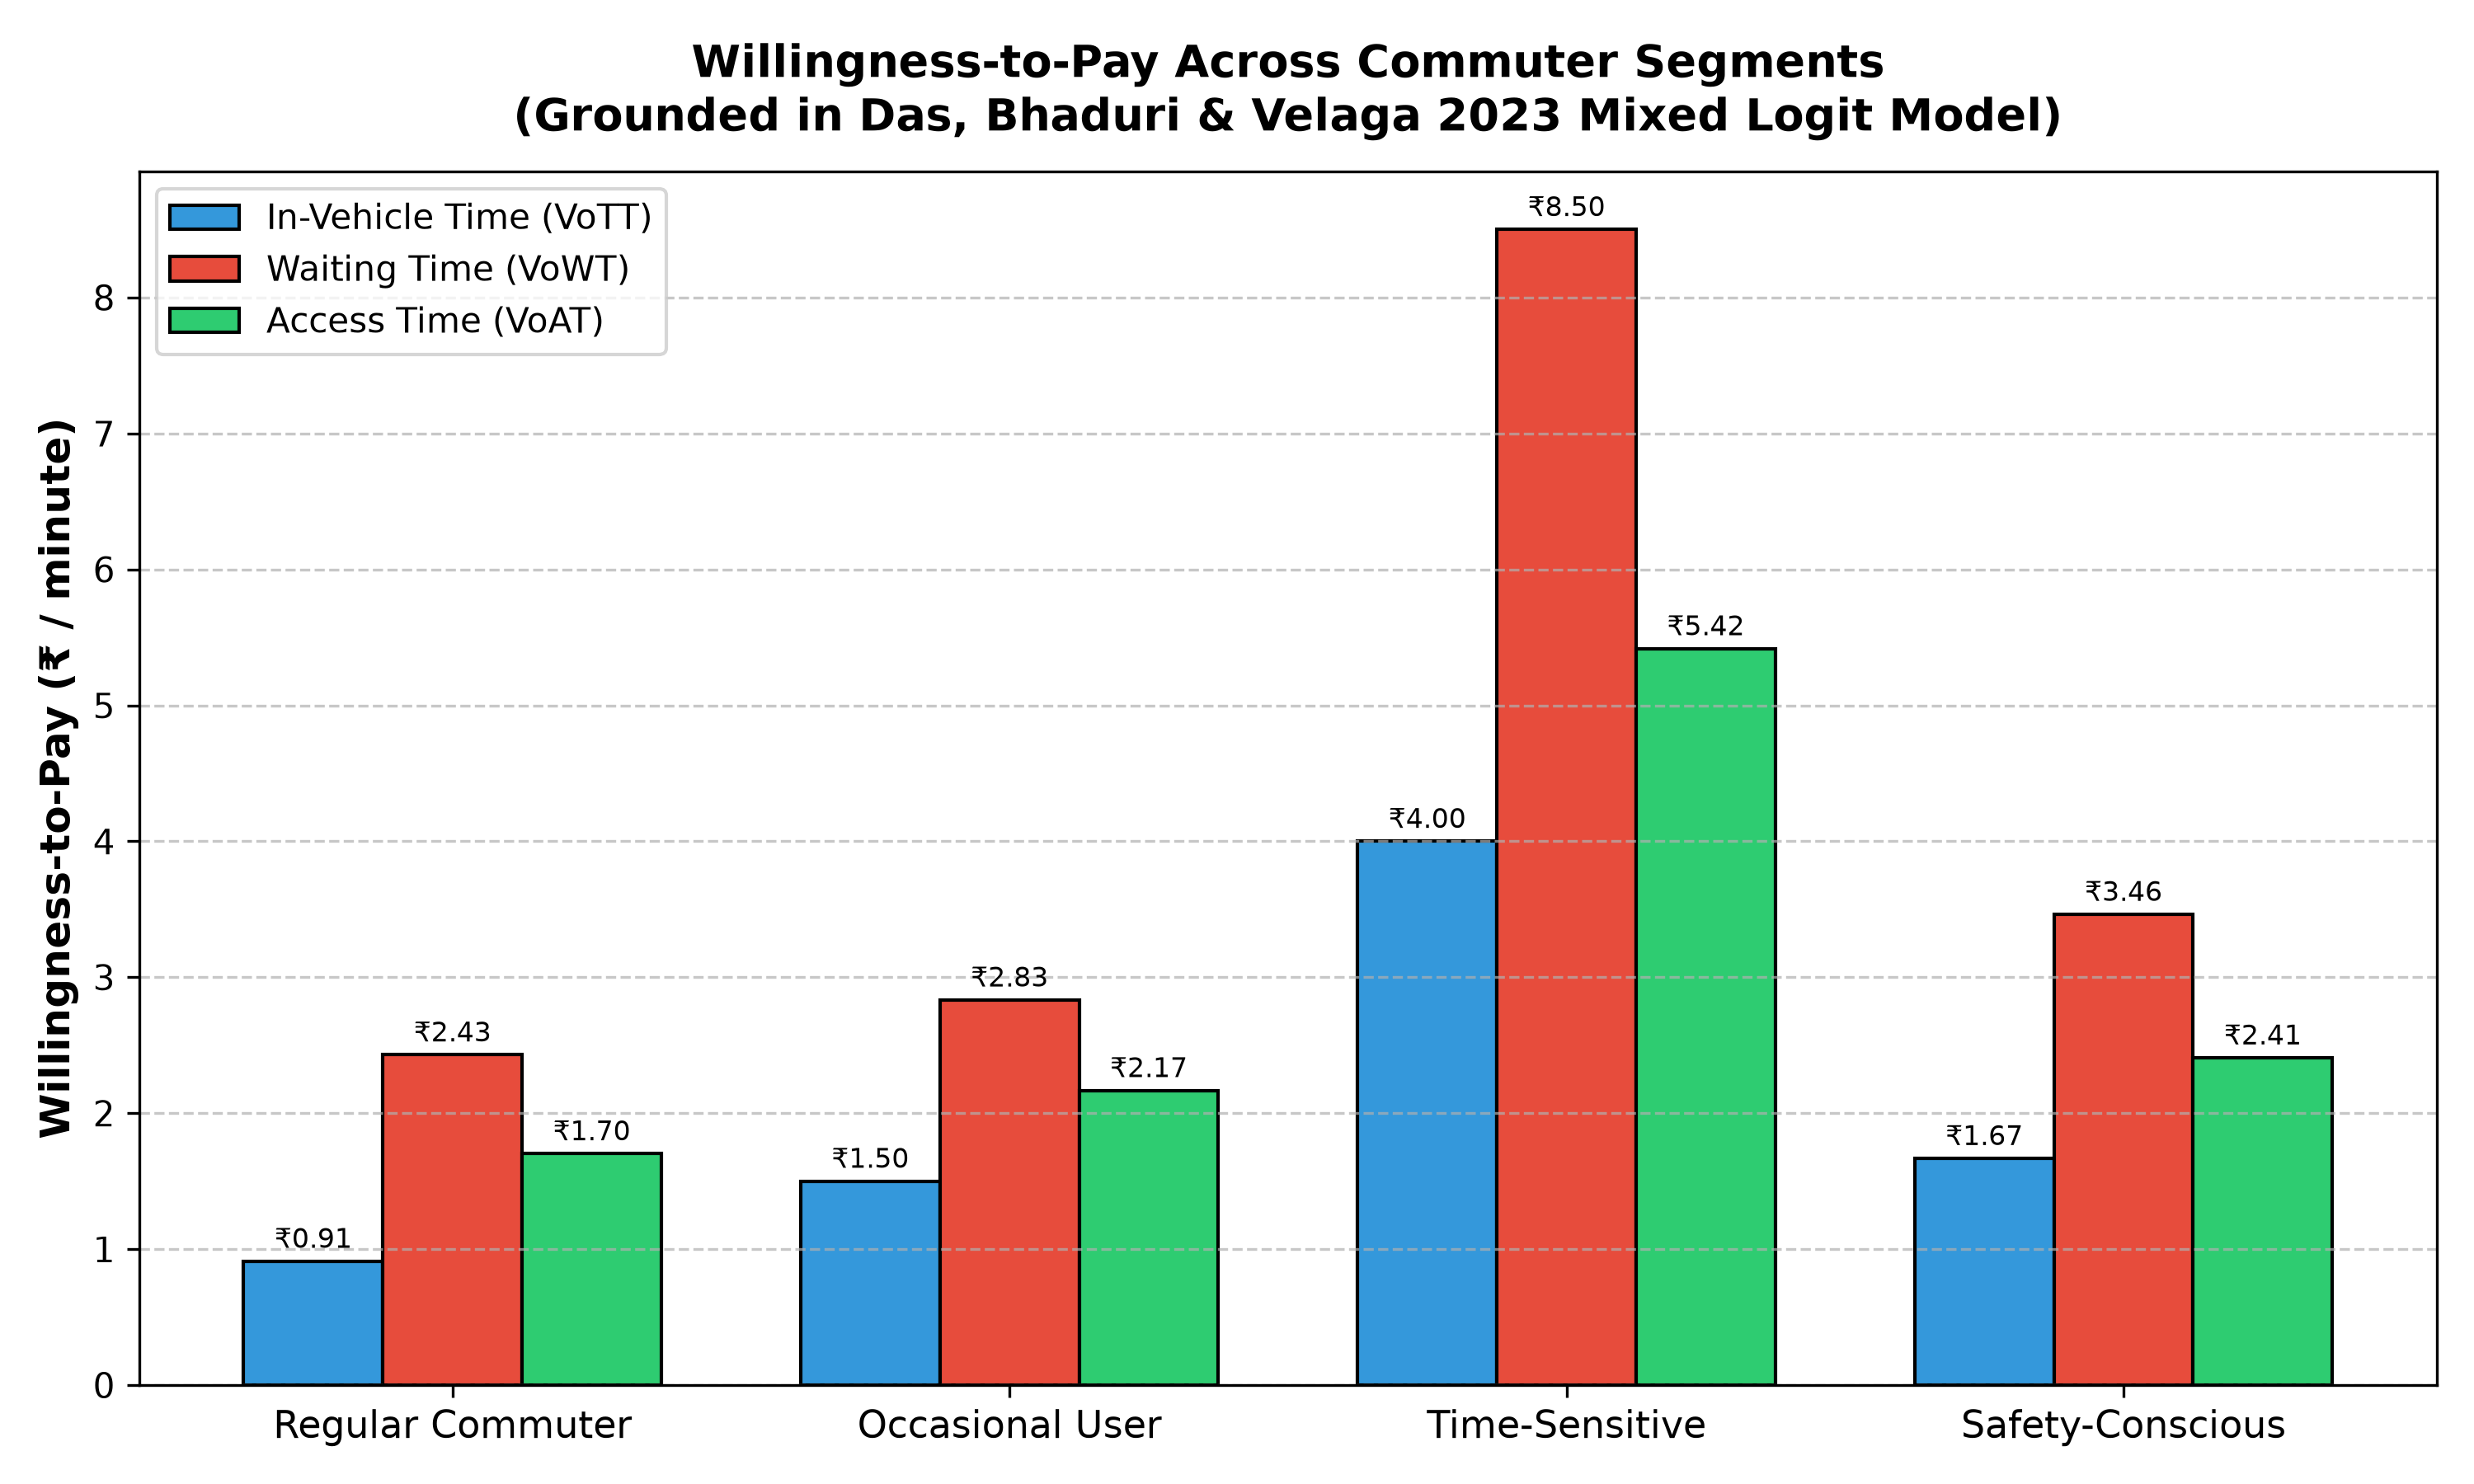
\includegraphics[width=0.82\linewidth]{figures/wtp_by_segment.png}
\caption{Empirical Willingness-to-Pay distributions across passenger segments derived from Das et al. (2023).}
\label{fig:wtp-by-segment}
\end{figure}

\section{Discussion}
The experimental results demonstrate a decisive trade-off between vehicular sharing, passenger service rates, and trip detours:
\begin{enumerate}
\item \textbf{Capacity Multiplication Under Demand Stress:} Under high demand (150 requests), solo unshared dispatch (A2) collapses to an 18.7\% service rate because autos are locked into single-party direct trips. In contrast, Greedy (A4) and Regret (A5) insertion achieve a 44.0\% service rate---a 2.35$\times$ increase in throughput using the identical vehicle fleet.
\item \textbf{Sub-Linear Detour Inconvenience:} Interleaving pickups and dropoffs raises average passenger in-vehicle detour by only 15\% (Low tier) to 24\% (Medium tier). This modest detour enables significant fare reductions (down to \rupee149.7--\rupee162.0) while generating higher pooled revenue for the auto driver.
\item \textbf{Proven Near-Optimality of Insertion Heuristics:} On the exact benchmark instance, Greedy Insertion (A4) and Regret Insertion (A5) achieve an optimality gap of only \textbf{6.82\%} relative to the global theoretical optimum (A7). Both heuristics solve assignments in 1.33--1.75 milliseconds per request, making them suitable for real-time online dispatch.
\item \textbf{Commuter Segment Sensitivity:} When scored via generalized cost, the routing engine successfully reflects differing passenger priorities:
  \begin{itemize}
  \item \textbf{Time-Sensitive Commuters} achieve the lowest waiting time (3.71 minutes, a 48\% reduction over A3) because their high Value of Waiting Time (\rupee8.50/min) penalizes delayed dispatch.
  \item \textbf{Regular Commuters} minimize generalized cost (\rupee202.75) by balancing minor detour with fare savings.
  \item \textbf{Safety-Conscious Commuters} achieve competitive service rates (65.0\%) while explicitly avoiding vehicles operating above the 75\% crowding discomfort threshold.
  \end{itemize}
\end{enumerate}

\section{Limitations and Threats to Validity}
\begin{itemize}
\item \textbf{Synthetic Demand Generation:} Requests were generated using Poisson processes over regional hubs. Real-world demand exhibits spatial clustering, tidal commute flows, and unmodeled roadside physical hailing.
\item \textbf{Simplified Road Network:} The experimental graph uses 15 hubs and 50 corridors. While spatially representative of Bengaluru's arterial layout, intra-neighborhood local streets and intersection delay dynamics are omitted.
\item \textbf{Constant Speed Assumption:} Edge travel times are calculated from free-flow speeds (25--42\,km/h) without dynamic peak-hour congestion feedback or live traffic sensor integration.
\item \textbf{Static Preference Parameters:} The Mixed Logit coefficients derived from Das et al. (2023) were measured in the Mumbai Metropolitan Region. While structurally applicable to Indian paratransit, localized calibration for Bengaluru commuters remains future work.
\item \textbf{Deterministic Driver Acceptance:} Vehicles are modeled as cooperative agents adhering strictly to assigned schedules. Real-world driver refusal, route deviation, and fare bargaining are not simulated.
\end{itemize}

\section{Summary}
This chapter designed, implemented, and empirically evaluated a Dynamic Dial-a-Ride (D-DARP) flexible shared-auto paratransit routing engine for PUMO, incorporating modified GTFS paratransit corridor models (Williams et al., 2015), Mixed Logit commuter preference structures (Das et al., 2023), and nonlinear crowding discomfort penalties (Das and Mandal, 2021).

Across identical demand tiers, combinatorial stop insertion (A4, A5) increased passenger service rate by up to 2.35$\times$ over solo ride-hail baselines while constraining average trip detour to 15--24\%. Benchmarked against a branch-and-bound global optimum solver (A7), the insertion heuristics demonstrated an optimality gap of only 6.82\% with an average runtime of under 2 milliseconds per request. Furthermore, preference-weighted assignment successfully aligned routing decisions with commuter priorities, reducing waiting times for time-sensitive riders to 3.71 minutes and optimizing generalized costs for regular commuters.
